% Version 2022-09-20
% update – 161114 by Ken Arroyo Ohori: made spacing closer to Word template throughout, put proper quotes everywhere, removed spacing that could cause labels to be wrong, added non-breaking and inter-sentence spacing where applicable, removed explicit newlines
% update – 010819 by Dennis Wittich: made spacing and font size closer to Word template, updated references and refernces style
% update – 042319 by Dennis Wittich: font size of captions set to 'small', first author names are shortened, hyphenation fixed
% update – 010620 by Dennis Wittich: Footnotes alignment set to left
% update - 151220 by Clement Mallet: Template adapted for double blind full paper submissions
% update - 060321 by Christian Heipke: Template refined for double blind full paper submissions
% update - 090921 by Christian Heipke: Template refined for double blind full paper submissions
% update - 200922 by Christian Heipke: general template update
% update - 080124 by Christian Heipke: general template update

\documentclass{isprs} % isprs class modified 23-04-2019 (Dennis Wittich)
\usepackage{subfigure}
\usepackage{setspace}
\usepackage{geometry} % added 27-02-2014 Markus Englich
\usepackage{epstopdf}
\usepackage[labelsep=period]{caption}  % added 14-04-2016 Markus Englich - Recommendation by Sebastian Brocks
\usepackage[british]{babel} 
\usepackage[hang]{footmisc}
\def\footnotemargin{1em} % added 08-01-2020 Dennis Wittich

%\usepackage[authoryear]{natbib}
%\def\bibhang{0pt}

\geometry{a4paper, top=25mm, left=20mm, right=20mm, bottom=25mm, headsep=10mm, footskip=12mm} % added 27-02-2014 Markus Englich
%\usepackage{enumitem}

%\usepackage{isprs}
%\usepackage[perpage,para,symbol*]{footmisc}

%\renewcommand*{\thefootnote}{\fnsymbol{footnote}}
\captionsetup{justification=centering,font=normal} % thanks to Niclas Borlin 05-05-2016
\captionsetup[figure]{font=small} % added 23-04-2019 Dennis Wittich
\captionsetup[table]{font=small} % added 23-04-2019 Dennis Wittich

\begin{document}

\title{Automatic Tree Segmentation for a ULS Point Cloud of a Forest}
\date{31.03.2025}


% KAO: Remove extra spacing

% Anonymous submissions, authors' names should not be visible
% \author{
%  Orhan Altan\textsuperscript{1}, Ian Dowman\textsuperscript{2}, Florent Lafarge\textsuperscript{3}, Clément Mallet\textsuperscript{4}, Christian Heipke\textsuperscript{5} }
\author{Runan Dunan\textsuperscript{1}, Anne Heichen\textsuperscript{2}}

% KAO: Remove extra newline
% Anonymous submissions, authors' affiliations should not be visible
%\address{
%	\textsuperscript{1 }ITU, Civil Engineering Faculty, 80626 Maslak Istanbul, Turkey - (oaltan, tozg, kulur, seker)@itu.edu.tr\\
%	\textsuperscript{2 }Dept.\ of Geomatic Engineering, University College London, Gower Street, London, WC1E 6BT UK - idowman@ge.ucl.ac.uk\\
%	\textsuperscript{3 }Université Côte d’Azur, INRIA – Sophia-Antipolis, France – florent.lafarge@inria.fr\\
%	\textsuperscript{4 }Univ. Gustave Eiffel, IGN-ENSG, LaSTIG – Saint-Mandé, France – clement.mallet@ign.fr\\
%	\textsuperscript{5 }Institute of Photogrammetry and GeoInformation, Leibniz Universit\"at Hannover, Germany - heipke@ipi.uni-hannover.de\\
%}
\address{\textsuperscript{1 }University of Heidelberg – mail@stud.uni-heidelberg.\\
{2 }University of Heidelberg – anne.heichen@stud.uni-heidelberg.\\}

% If the corresponding author is NOT the final author, always add a % space before the subsequent comma, i.e.
% first author name\textsuperscript{a,}\thanks{Corresponding author} , % second author name \textsuperscript{b}, etc.
% thanks to Niclas Borlin 05-05-2016
% information on the corresponding author should not be used any longer and has been commented out
% C. Heipke, Jan 03,2024

% the use of the information of commissions and working groups should not be used any longer and has been commented out
% C. Heipke, Sept. 20,2022
%\commission{XX, }{YY} %This field is optional. If filled, XX and YY should be replaced by adequate numbers. See https://www2.isprs.org/commissions/
%\workinggroup{XX/YY} %This field is optional.
%\icwg{}   %This field is optional.


% KAO: Use times symbol
\abstract{

100-250 words: Lorem ipsum dolor sit amet, consetetur sadipscing elitr, sed diam nonumy eirmod tempor invidunt ut labore et dolore magna aliquyam erat, sed diam voluptua. At vero eos et accusam et justo duo dolores et ea rebum. Stet clita kasd gubergren, no sea takimata sanctus est Lorem ipsum dolor sit amet. Lorem ipsum dolor sit amet, consetetur sadipscing elitr, sed diam nonumy eirmod tempor invidunt ut labore et dolore magna aliquyam erat, sed diam voluptua. At vero eos et accusam et justo duo dolores et ea rebum. Stet clita kasd gubergren, no sea takimata sanctus est Lorem ipsum dolor sit amet. Lorem ipsum dolor sit amet, consetetur sadipscing elitr, sed diam nonumy eirmod tempor invidunt ut labore et dolore magna aliquyam erat, sed diam voluptua. At vero eos et accusam et justo duo dolores et ea rebum. Stet clita kasd gubergren, no sea takimata sanctus est Lorem ipsum dolor sit amet.   
Duis autem vel eum iriure dolor in hendrerit in vulputate velit esse molestie consequat, vel illum dolore eu feugiat nulla facilisis at vero eros et accumsan et iusto odio dignissim qui blandit praesent luptatum zzril delenit augue duis dolore te feugait nulla facilisi. Lorem ipsum dolor sit amet, \\ \\
whole paper max. 8 pages excluding references


}

\keywords{LiDAR, Tree Segmentation, ULS, max. 6}

\maketitle
% KAO: Sloppy spacing ensures non-overfull lines. Can be removed if this is not an issue.
\sloppy


\section{Introduction}\label{Introduction}

 Relevance of the topic in general and in geography
 – Scope and definition of the specific topic
 – Objective of the specific paper / work → small research question!



\begin{itemize}
\setlength\itemsep{0em}\setlength\parskip{0em}\setlength\topsep{0em}\setlength\partopsep{0em}\setlength\parsep{0em} 
\item{Relevance of the topic in general and in geography} 
\item{Scope and definition of the specific topic}
\item{Objective of the specific paper / work → small research question!}
\end{itemize}

invidunt ut labore et dolore magna aliquyam erat, sed diam voluptua. At vero eos et accusam et justo duo dolores et ea rebum. Stet clita kasd gubergren, no sea takimata sanctus est Lorem ipsum dolor sit amet. Lorem ipsum dolor sit amet, consetetur sadipscing elitr, sed diam nonumy eirmod tempor invidunt ut labore et dolore magna aliquyam erat, sed diam voluptua. At vero eos et accusam et justo duo dolores et ea rebum. Stet clita kasd gubergren, no sea takimata sanctus est Lorem ipsum dolor sit amet. Lorem ipsum dolor sit amet, consetetur sadipscing elitr, sed diam nonumy eirmod tempor invidunt ut labore et dolore magna aliquyam erat, sed diam voluptua. At vero eos et accusam et justo duo dolores et ea rebum. Stet clita kasd gubergren, no sea takimata sanctus est Lorem ipsum dolor sit amet.   
Duis autem vel eum iriure dolor in hendrerit in vulputate velit esse molestie consequat, vel illum dolore eu feugiat nulla facilisis at vero eros et accumsan et iusto odio dignissim qui blandit praesent luptatum zzril delenit augue duis dolore te feugait nulla facilisi. Lorem ipsum dolor sit amet,


\section{State of the Art}\label{State of the Art}

– Current aspects of the topic under research
– Overview about different methods
– Related applications examples

\begin{itemize}
\setlength\itemsep{0em}\setlength\parskip{0em}\setlength\topsep{0em}\setlength\partopsep{0em}\setlength\parsep{0em} 
\item{Current aspects of the topic under research} 
\item{Overview about different methods}
\item{Related applications examples}
\end{itemize}

Lorem ipsum dolor sit amet, consetetur sadipscing elitr, sed diam nonumy eirmod tempor invidunt ut labore et dolore magna aliquyam erat, sed diam voluptua. At vero eos et accusam et justo duo dolores et ea rebum. Stet clita kasd gubergren, no sea takimata sanctus est Lorem ipsum dolor sit amet. Lorem ipsum dolor sit amet, consetetur sadipscing elitr, sed diam nonumy eirmod tempor invidunt ut labore et dolore magna aliquyam erat, sed diam voluptua. At vero eos et accusam et justo duo dolores et ea rebum. Stet clita kasd gubergren, no sea takimata sanctus est Lorem ipsum dolor sit amet. Lorem ipsum dolor sit amet, consetetur sadipscing elitr, sed diam nonumy eirmod tempor invidunt ut labore et dolore magna aliquyam erat, sed diam voluptua. At vero eos et accusam et justo duo dolores et ea rebum. Stet clita kasd gubergren, no sea takimata sanctus est Lorem ipsum dolor sit amet.   
Duis autem vel eum iriure dolor in hendrerit in vulputate velit esse molestie consequat, vel illum dolore eu feugiat nulla facilisis at vero eros et accumsan et iusto odio dignissim qui blandit praesent luptatum zzril delenit augue duis dolore te feugait nulla facilisi. Lorem ipsum dolor sit amet,


\section{Data and Method}\label{Data and Method}



\begin{itemize}
\setlength\itemsep{0em}\setlength\parskip{0em}\setlength\topsep{0em}\setlength\partopsep{0em}\setlength\parsep{0em} 


\item{Description of the dataset used in the analysis} 
\item{Detailed explanation of the used methods and algorithm: How does it work? What are input and output data? Which parameters are required, which settings are used?}

\end{itemize}

Lorem ipsum dolor sit amet, consetetur sadipscing elitr, sed diam nonumy eirmod tempor invidunt ut labore et dolore magna aliquyam erat, sed diam voluptua. At vero eos et accusam et justo duo dolores et ea rebum. Stet clita kasd gubergren, no sea takimata sanctus est 

\subsection{Dataset}\label{sec:Dataset}

The data set used in this study consists of a point cloud of UAV-borne laser scanning (ULS) acquired in a forest environment~\cite{Weiser2022a}, which is displayed in Figure~\ref{fig: study area}. Data were collected in September 2019 under leaf-on conditions, covering a 1-hectare section of the Bretten municipal forest in Baden-Württemberg~\cite{Weiser2022b}. This site is a managed forest with a multi-layered canopy and a diverse species composition, including beech, spruce, Douglas fir, oaks, and European hornbeam, featuring dense canopy coverage~\cite{Weiser2022a}. The study area is characterised by undulating terrain in a hilly landscape typically for the Kraichgau region~\cite{Weiser2022c, Zhang2024}. This site is influenced by a temperate maritime climate with annual precipitation ranging from 41 to 63 mm and a growing season extending up to seven months~\cite{Zhang2024}. 

\begin{figure}[ht!]
\begin{center}
		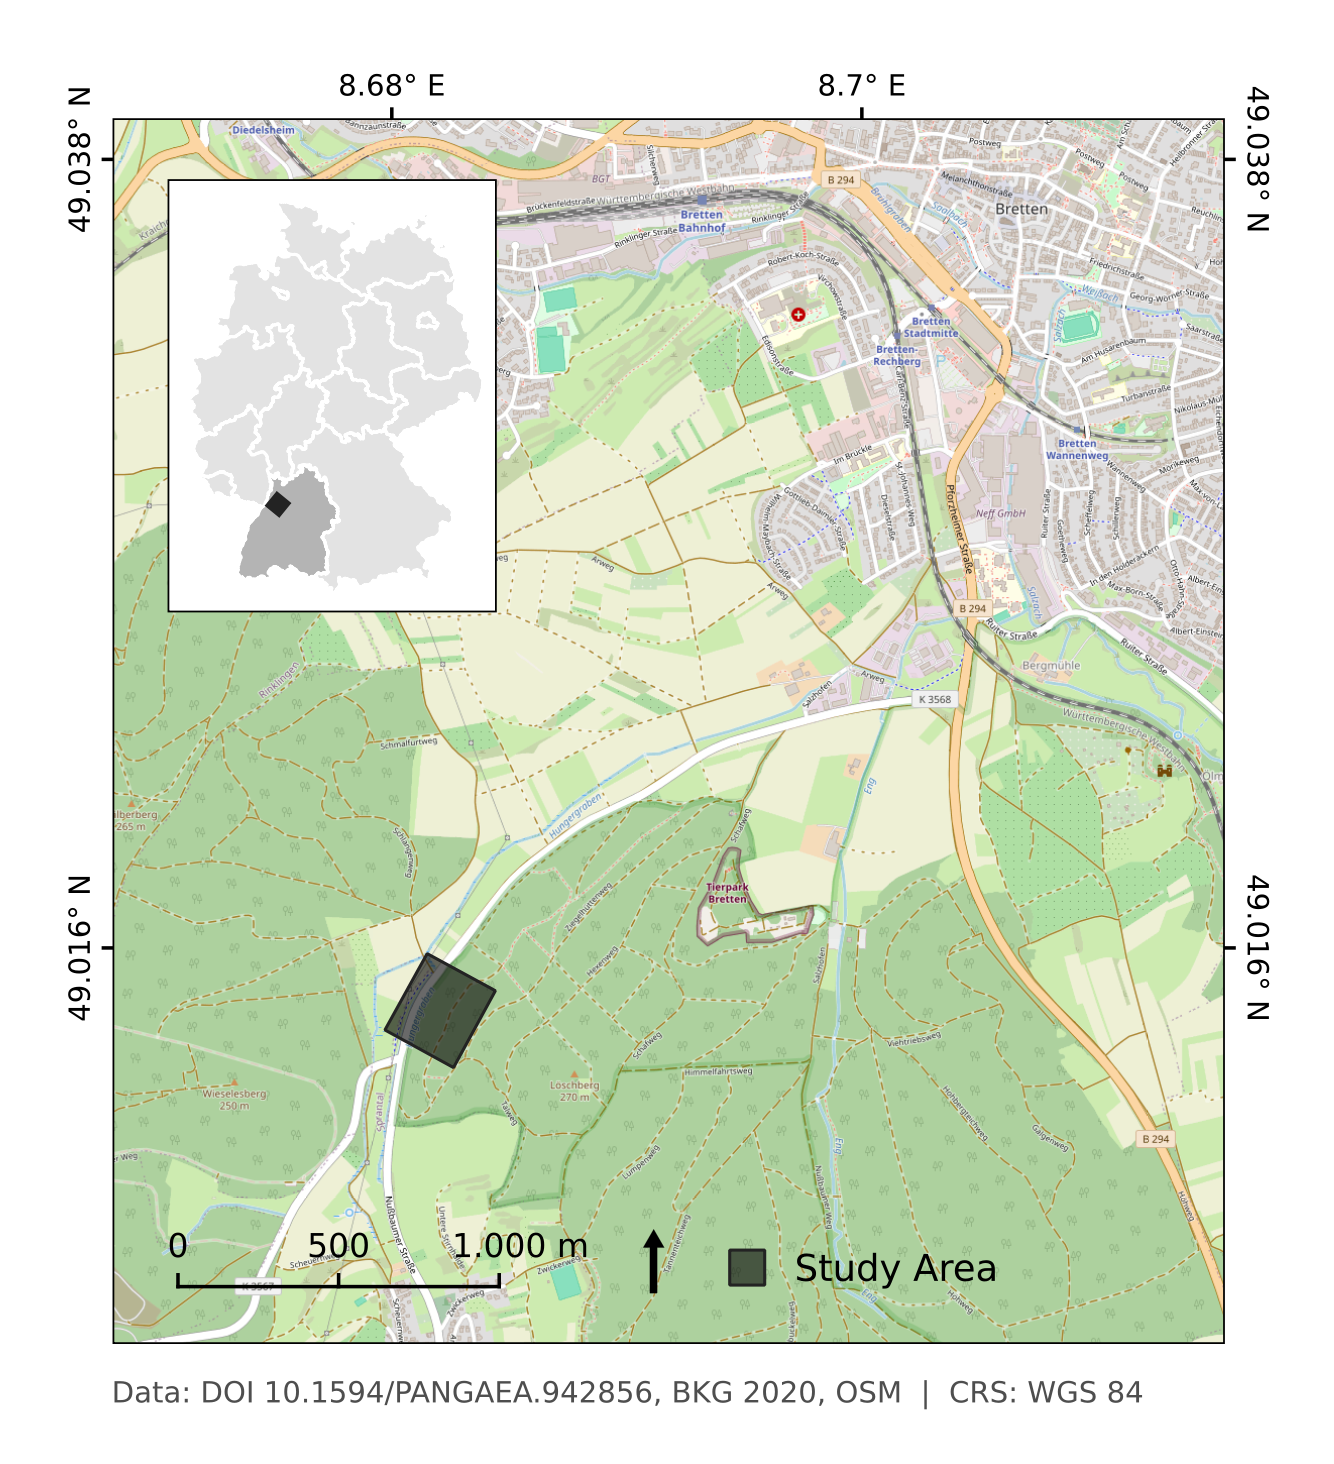
\includegraphics[width=1.0\columnwidth]{figures/study_area_map.png}
	\caption{Location of the study site near Bretten within Baden-Württemberg, Germany.}
\label{fig: study area}
\end{center}
\end{figure}

The sensor used for data acquisition was a RIEGL miniVUX-1UAV, which was mounted on a DJI Matrice 600 Pro drone, following a predefined flight plan. This plan consisted of two overlapping grid patterns, with the second grid rotated by 45 ° to enhance the variety of viewing angles. Each grid contained both parallel and orthogonal flight paths, ensuring comprehensive coverage of the forest structure~\cite{Weiser2022b}. The nominal specifications of the sensor can be found in Table~\ref{tab:instrument_specifications} by~\cite{Weiser2022b}.

\begin{table}[ht!]
    \centering
    \small
    \begin{tabular}{|l|l|}
        \hline
        \textbf{Parameter} & \textbf{Specification} \\
        \hline
        Accuracy & 15 mm at 50 m scanning range \\
        Precision & 10 mm at 50 m scanning range \\
        Laser beam divergence & 1.6 × 0.5 mrad, full width measured \\ & 50 \% peak intensity (FWHM) \\
        Scanning mechanism & Rotating mirror \\
        \hline
    \end{tabular}
    \caption{Instrument specifications for RIEGL miniVUX-1UAV~\protect\cite{Weiser2022b}.}
\label{tab:instrument_specifications}
\end{table}

The ULS data processing was carried out by the 3DGeo Research Group Heidelberg. The trajectory was estimated using PPK GNSS from SAPOS Baden-Württemberg with a Virtual Reference Station and processed in ETRS89/UTM 32N. The data were imported into RiPROCESS version 1.4.2, converted to polar coordinates, and transformed to global coordinates. A strip adjustment was applied to refine the accuracy of the trajectory (considering points only with a scan angle \textless 45 ° off-nadir), and the final point cloud (only points with reflectance between -22 and +10 dB and range between 5 and 150 m) was exported in LAZ 1.4 format with the corresponding reflectance and waveform information. The flight strips were merged using LAStools version 200509, encoding flight line information. Quality control was conducted by using OPALS version 2.3.2.~\cite{Weiser2022b}.

For validation, 503 segmented trees from the ULS original dataset were used~\cite{Weiser2022a}. The segmentation was initially performed on terrestrial laser scanning (TLS) point clouds using CompuTree software and a Euclidean clustering approach combined with a competitive Dijkstra’s algorithm from the SimpleTree plugin. The method distinguished individual trees based on shortest-path computations and was refined through manual corrections to address errors from overlapping crowns and occlusions. The TLS-segmented trees served as a reference for manually adjusting the ULS-based segmentation. Extracted tree attributes included tree height, crown base height, crown projection area (based on the convex and the concave hull of crown points), crown diameter and stem diameter at breast height~\cite{Weiser2022b}.

\subsection{Methods}\label{sec:Method}



workflow shown in Figure~\ref{fig:figure workflow}

\begin{figure}[ht!]
\begin{center}
		
\includegraphics[width=1.0\columnwidth]{figures/test_sites/fig1.eps}
	\caption{Study area.}
\label{fig:figure workflow}
\end{center}
\end{figure}






\section{Results}\label{Results}


\begin{itemize}
\setlength\itemsep{0em}\setlength\parskip{0em}\setlength\topsep{0em}\setlength\partopsep{0em}\setlength\parsep{0em} 
\item{Discussion of results in the context of objective and state of the art} 
\end{itemize}



represented in equotation \ref{equ:1}
\begin{equation}\label{equ:1}
	x = x_0 -c \frac{X - X_0}{Z - Z_0}; y = y_0 -c \frac{Y - Y_0}{Z - Z_0},
\end{equation}




\section{Discussion and Conclusion}\label{Discussion and Conclusion}

\begin{itemize}
\setlength\itemsep{0em}\setlength\parskip{0em}\setlength\topsep{0em}\setlength\partopsep{0em}\setlength\parsep{0em} 
\item{Discussion of results in the context of objective and state of the art} 

\item{Most important findings of the analysis and regarding the method}
\end{itemize}




{
	\begin{spacing}{1.17}
		\normalsize
		\bibliography{automatic_tree_segmentation_authors}
	\end{spacing}
}

\end{document}

